\listoftodos


\chapter{Werkzeuge}
\label{chap:Werkzeuge}
Dieses Kapitel erläutert die erstellten Werkzeuge im Detail. Da die Werkzeuge auf einander aufbauen, werden sie der Reihe nach erläutert. 

	\section{ConvolutionalSecondCriterionAutoenocder}
	\label{sec:SecondCriterionAutoenocder}
	Der SCAE erweitert einen ConvolutionalAutoencoder um ein weiteres Kriterium. Es gibt also zusätzlich zu der Rekonstruktion des Autoencoders einen weiteren Ausgang. Der zweite Ausgang kann wie jeder Ausgang für eine Binärklassifikation, für eine Multiklassifikation oder für eine Regression genutzt werden. In Abbildung \ref{img:SchemaSCAE} ist der schematische Aufbau des SCAE abgebildet. Die Schichten der zweiten Aufgabe gehen von dem Code-Layer ab. Es können belibig viele Schichten angehängt werden. Die Verlustfunktion des NN besteht aus der Summe der einzelnen Verlustfunktionen und einer Gewichtung. Sie lautet im Detail: 
	\begin{align}
	loss = weight1 * loss\_autoencoder + weight2 * loss\_secondcriterion
	\end{align}
	Die Gewichtung der Verlustfunktionen kann dem SCAE per Konstruktor-Argument übergeben werden. Das Werkzeug ist als Python-Module implementiert. Dabei implementiert die Klasse ConvolutionalSecondCriterionAutoenocder den ConvolutionalAutoenocder aus Psipy. In Abbildung \ref{img:KlassendiagrammCSCAE} ist das Klassendiagramm des SCAE dargestellt.
	\begin{figure}[h]
		\centering
		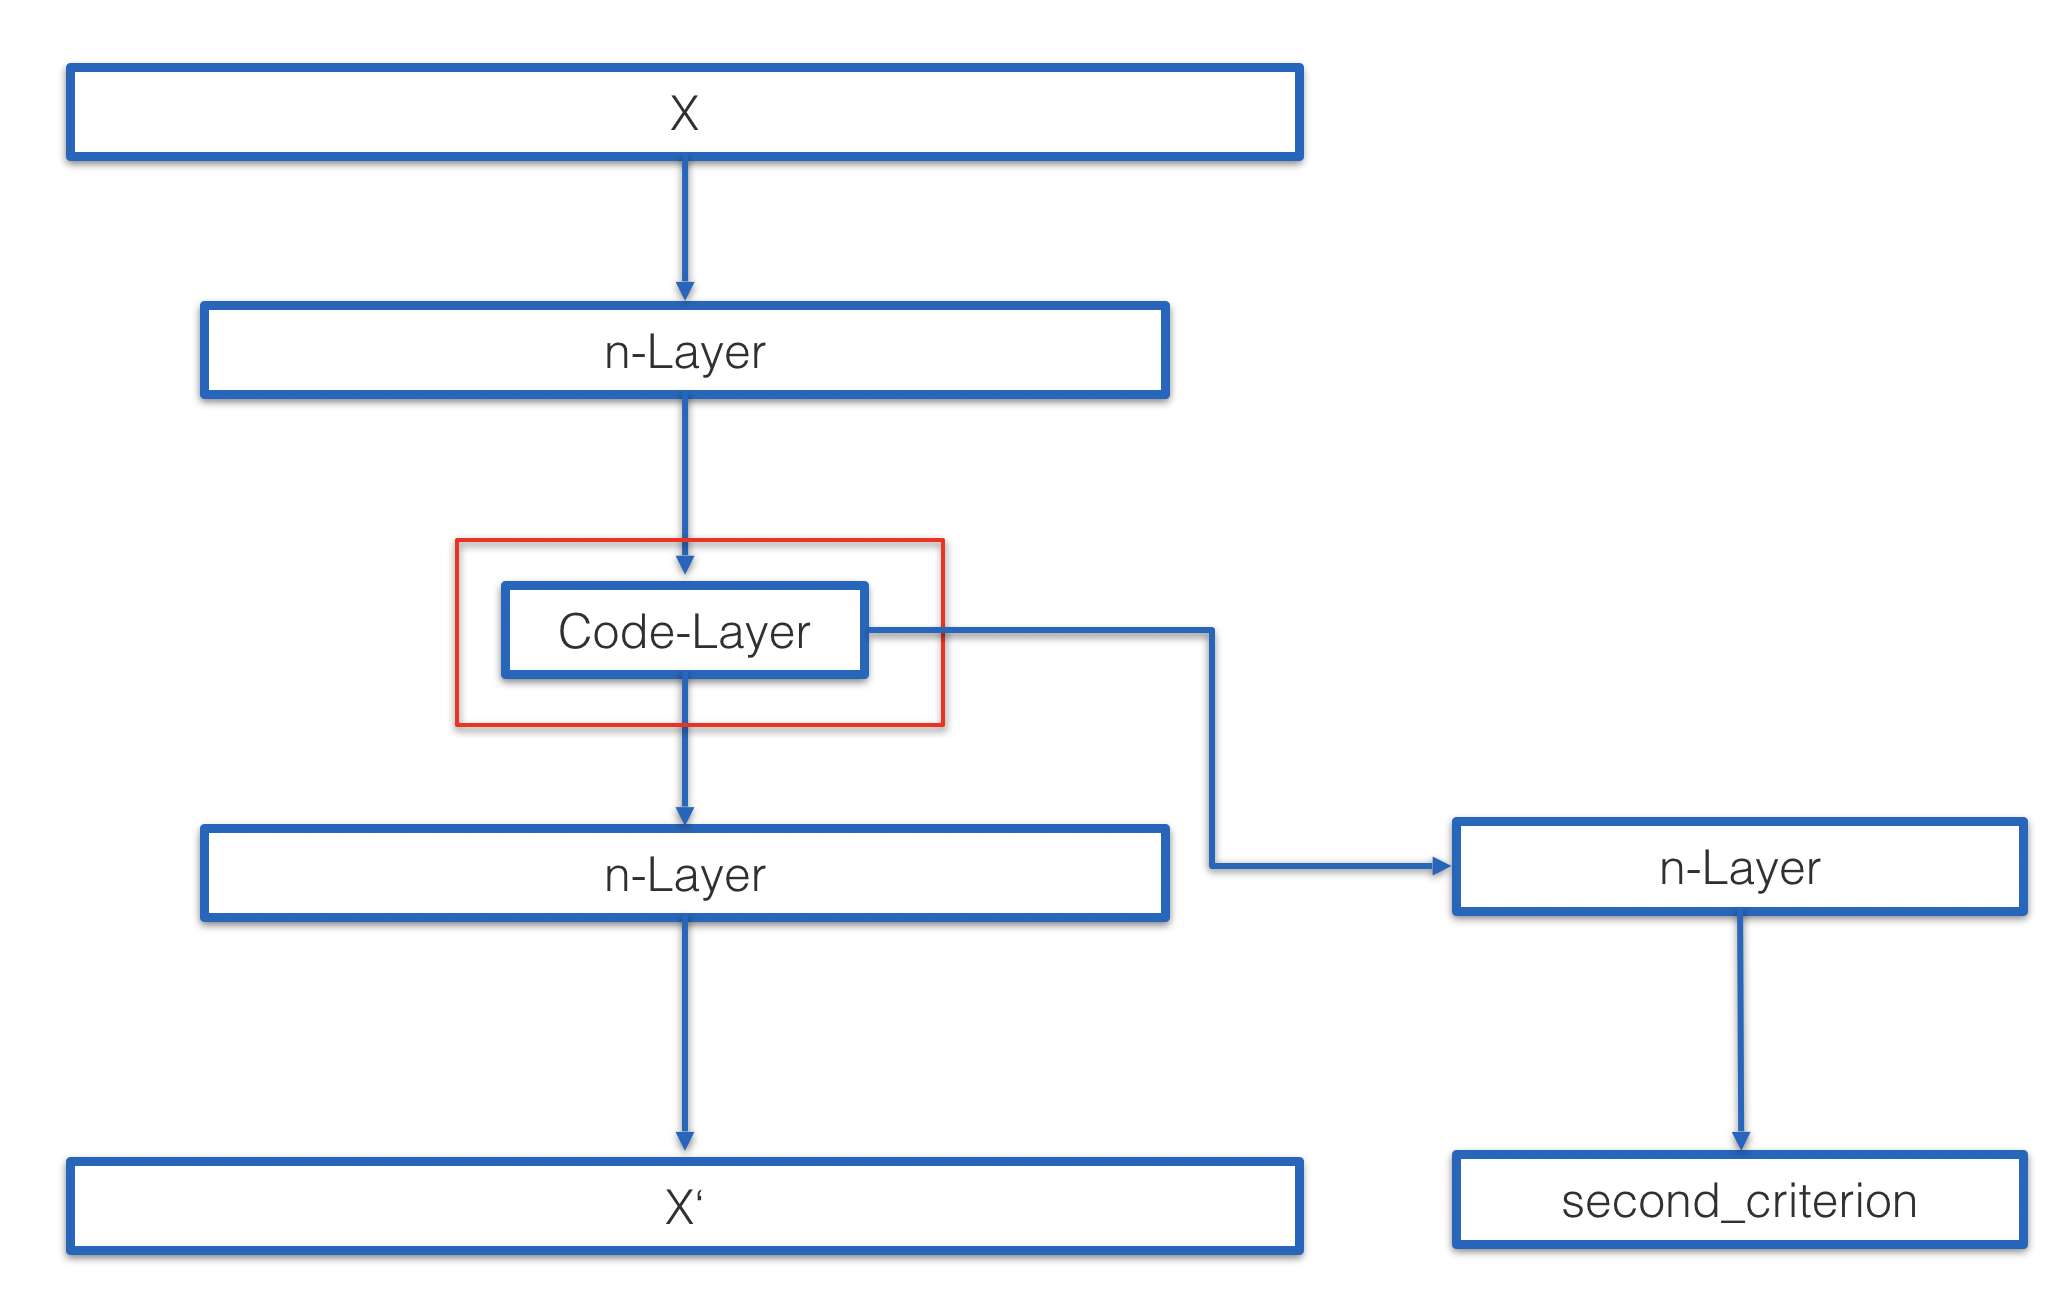
\includegraphics[width=0.5\textwidth, center]{bilder/Schema_Autoencoders/Schema_SCAE.png}
		\caption[Schema SecondCriterionAutoenocder]{Schema SecondCriterionAutoenocder}
		\label{img:SchemaSCAE}
	\end{figure}  
	\begin{figure}[h]
		\centering
		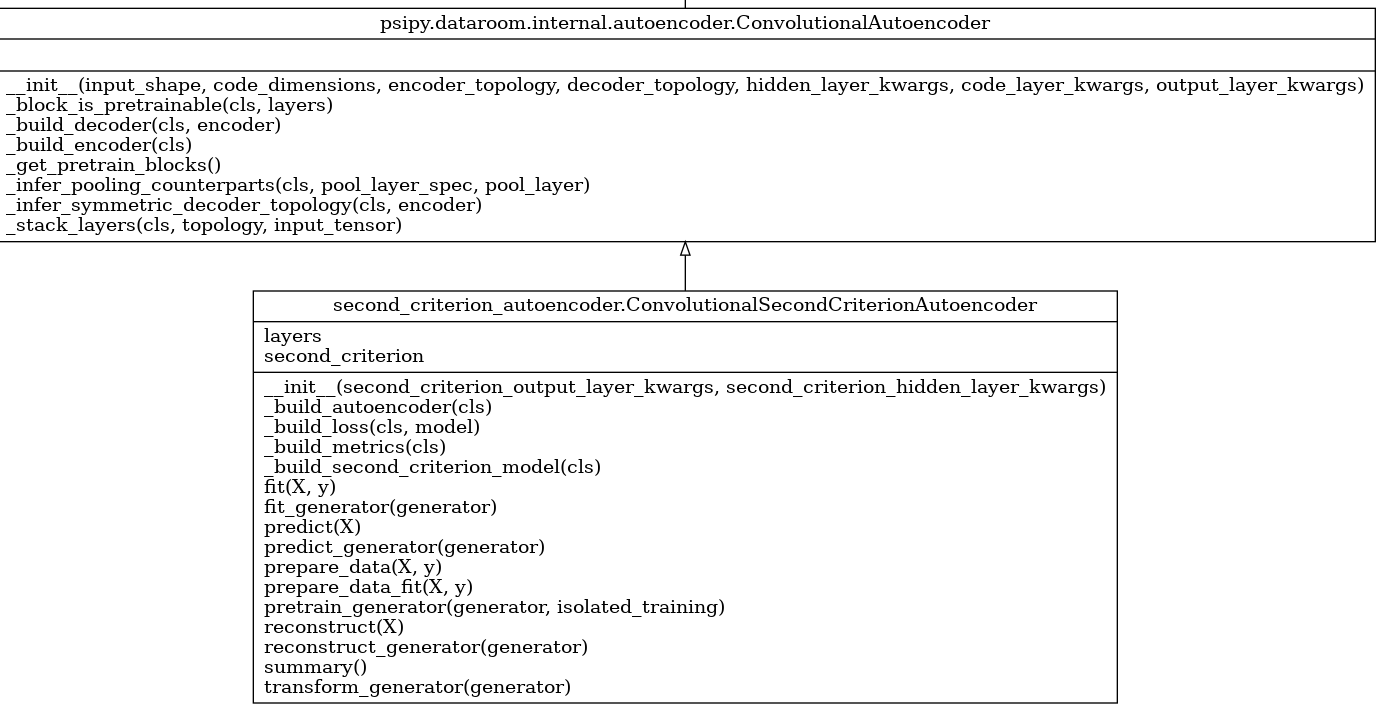
\includegraphics[width=0.5\textwidth, center]{bilder/Klassendiagramme/Klassendiagramm_CSCAE.png}
		\caption[Klassendiagramm ConvolutionalSecondCriterionAutoencoder]{Klassendiagramm ConvolutionalSecondCriterionAutoencoder}
	    \label{img:KlassendiagrammCSCAE}
	\end{figure}  
    Über den Konstruktor können alle Argumente welche zum Erstellen des Models notwendig sind per doppeltes Sternchen Wörterburch Argument (**kwargs) an die Klasse übergeben werden. Diese Technik erlaubt es eine mit Schlüsselwörtern versehene Argumentliste variabler Länge zu übergeben.  Die Argumentlisten  werden beinahe in allen Methode zum Einsatz gebracht. Sie werden insbesodnere genutzt um Argumente an die zugehörigen Keras-Methoden zu übergeben. Die Namensgebung der Methode orientiert sich dabei an Keras. So wird z.B. in dem Methodenaufruf $fit()$ unter anderem auch die Keras-Methode  $fit()$ aufgerufen. Um einen SCAE zu trainieren ist es notwendig einen Instanz zu erzeugen, die Methode $pretrain$ aufzurufen und ihn Anschliesend mit der Methode $fit$ zu trainieren.
    In dem Methodenaufruf $pretrain$ wird das Modell erstellt und Schichtenweise vortrainiert. Das eigentliche Trianing erfolgt in der MEthode $fit$. Alternativ können auch die zugehörigen generatorenklassen aufgerufen werden.
    
    
    In Listing xyz ist ein Beispielhafter Einsatz des SCAE dargestellt.


	\section{TransferSecondCriterionAutoenocder}
	\label{sec:TransferSecondCriterionAutoenocder}

	\begin{figure}[h]
		\centering
		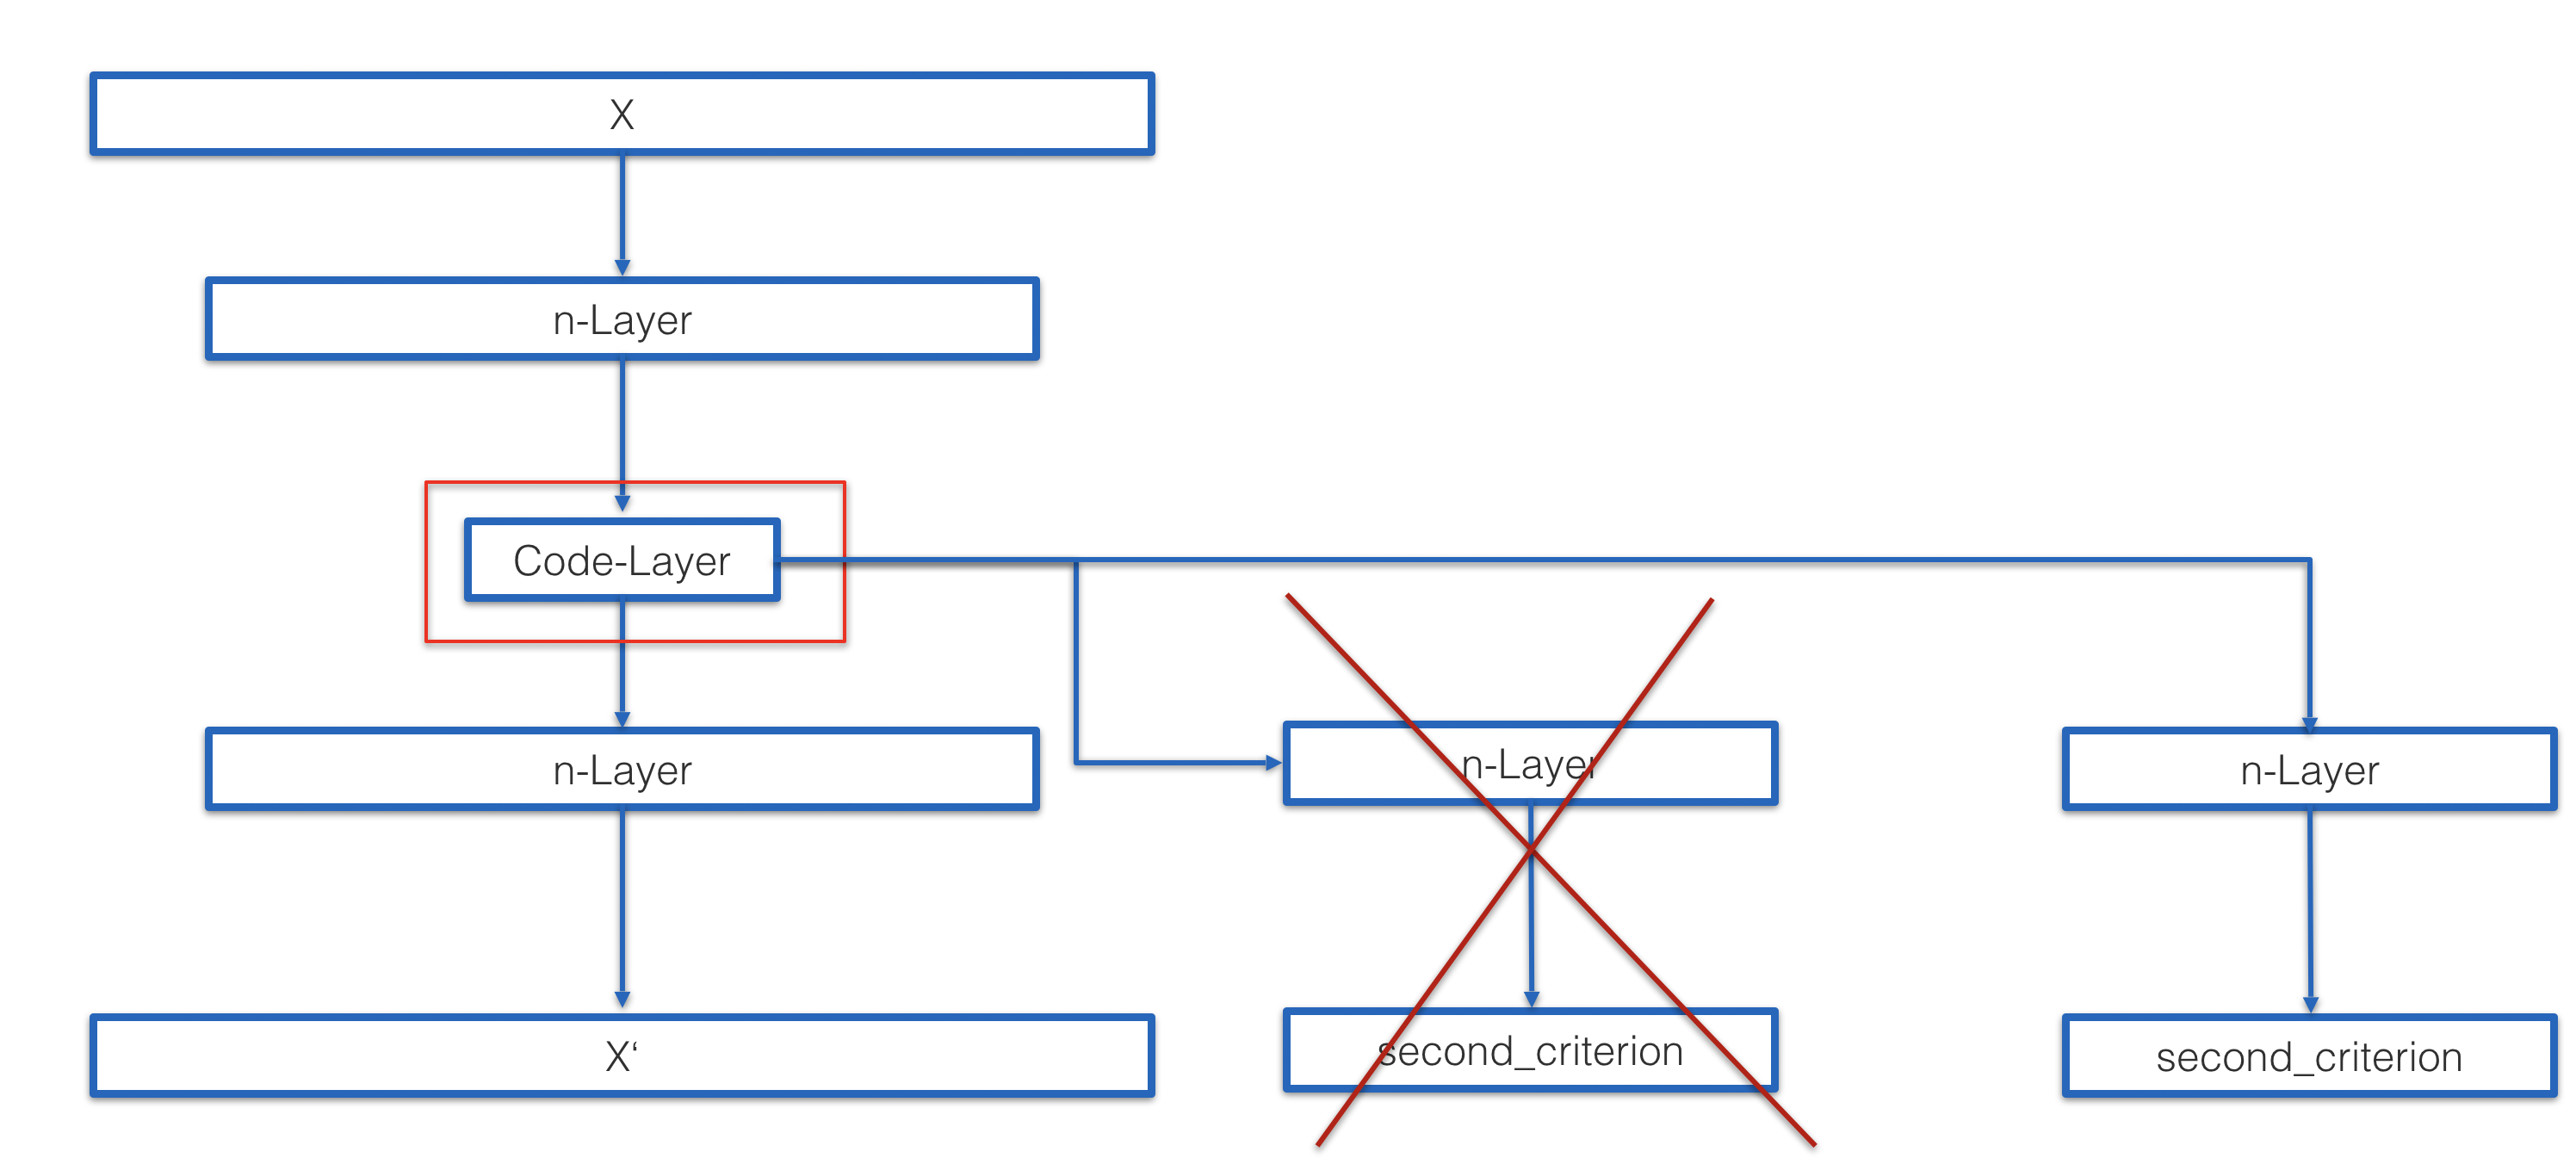
\includegraphics[width=0.5\textwidth, center]{bilder/Schema_Autoencoders/Schema_TSCAE.png}
		\caption[Schema TransferSecondCriterionAutoenocder]{Schema TransferSecondCriterionAutoenocder}
		\label{img:SchemaTSCAE}
	\end{figure}  

	
	\begin{figure}[h]
		\centering
		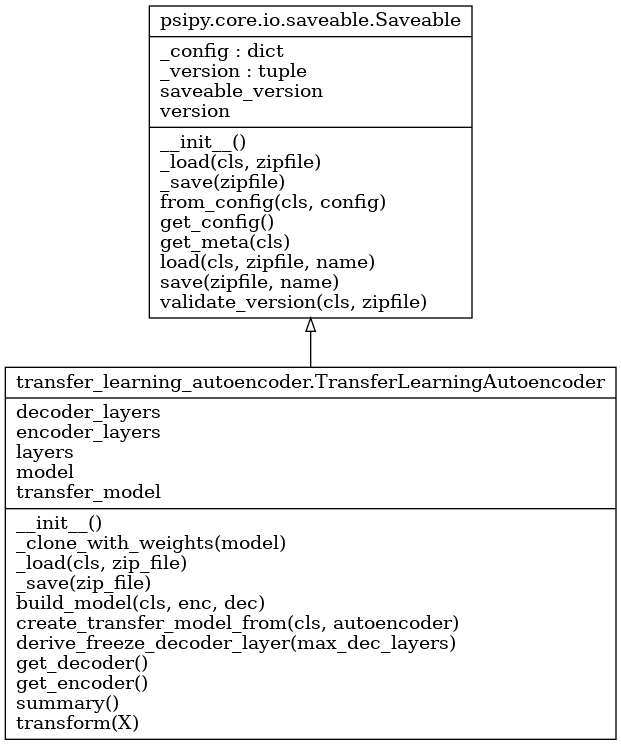
\includegraphics[width=0.5\textwidth, center]{bilder/Klassendiagramme/Klassendiagramm_TLCSCAE.png}
		\caption[Klassendiagramm TransferSecondCriterionAutoenocder]{Klassendiagramm TransferSecondCriterionAutoenocder}
		\label{img:KlassendiagrammTransferSecondCriterionAutoenocder}
	\end{figure}  
			
	\section{AutoTransferSecondCriterionAutoenocder}
	\label{sec:AutoTransferSecondCriterionAutoenocder}


	\begin{figure}[h]
		\centering
		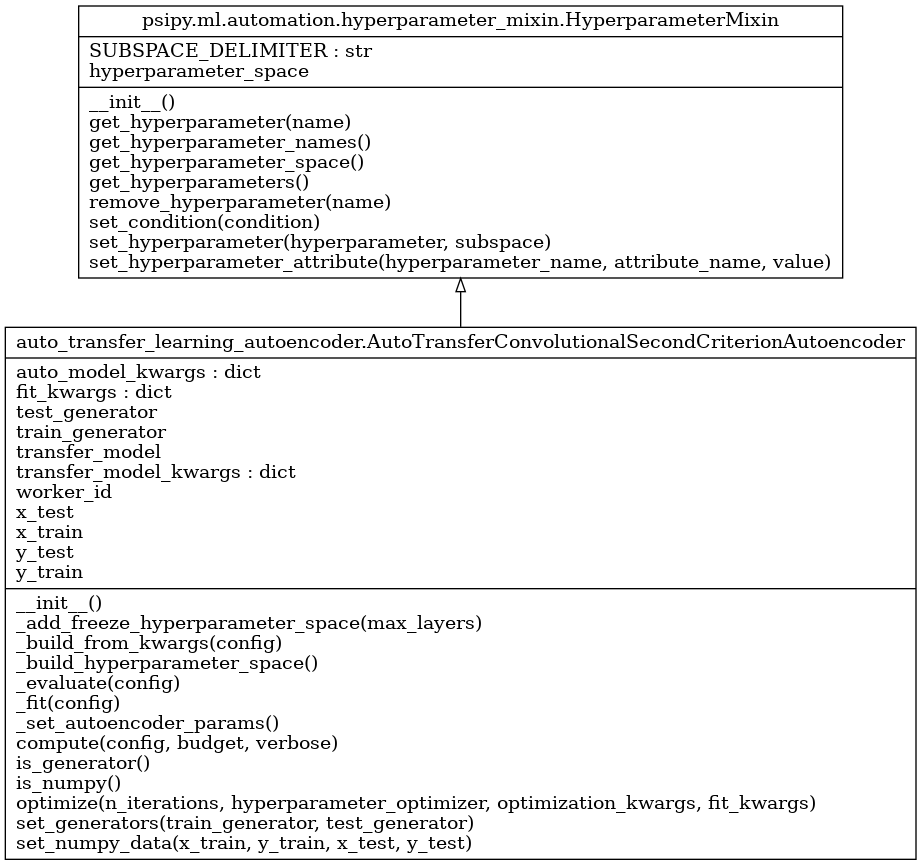
\includegraphics[width=0.5\textwidth, center]{bilder/Klassendiagramme/Klassendiagramm_AutoTLCSCAE.png}
		\caption[Klassendiagramm AutoTransferSecondCriterionAutoenocder]{Klassendiagramm AutoTransferSecondCriterionAutoenocder}
		\label{img:KlassendiagrammAutoTransferSecondCriterionAutoenocder}
	\end{figure}  